\usetikzlibrary{decorations.pathreplacing}

\begin{frame} %{overlapping registers (1)}
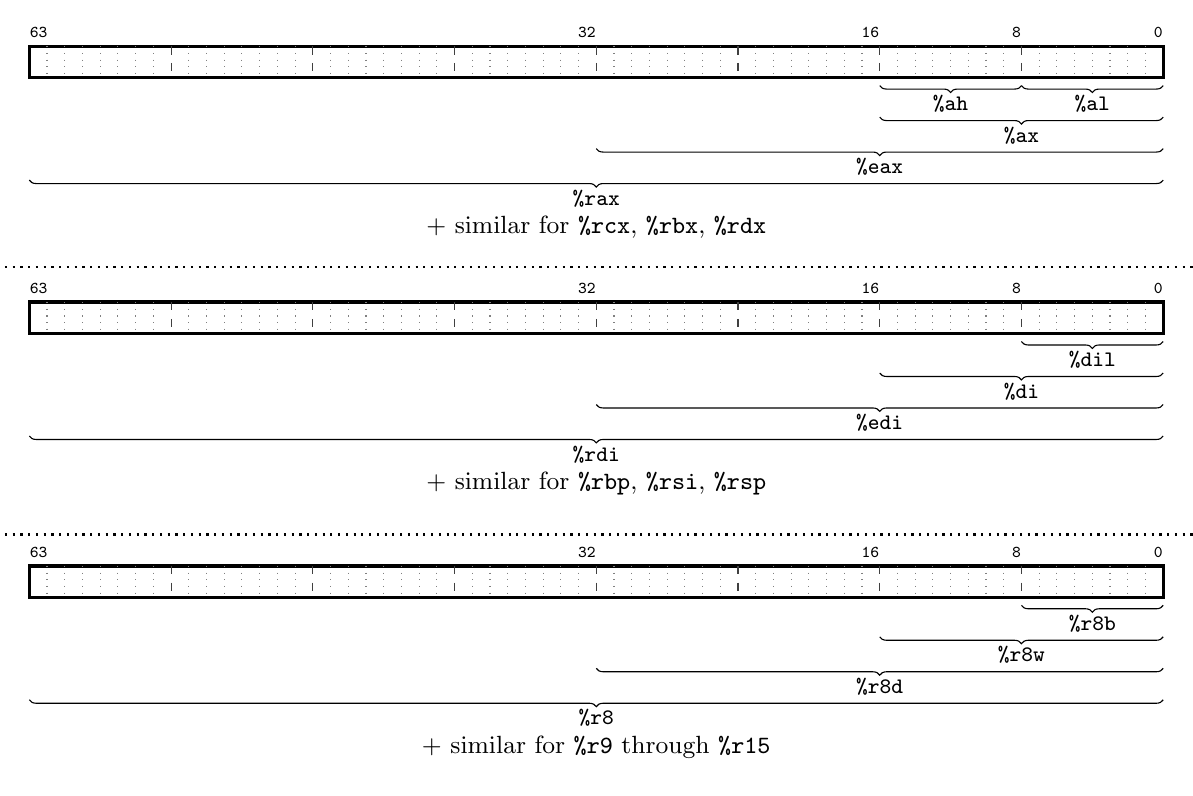
\begin{tikzpicture}
    \tikzset{
        main reg/.style={draw,very thick},
        reg label/.style={font=\fontsize{8.5}{9.5}\tt},
        bit label/.style={font=\fontsize{6}{7}\tt,inner sep=0mm,yshift=1mm},
        reg divider/.style={draw,thin,dashed,black!75},
        reg divider minor/.style={draw,thin,dotted,black!50},
    }
    \draw[overlay,thick,dotted] (-1, -2.8) -- ++(16, 0);
    \draw[overlay,thick,dotted] (-1, -6.2) -- ++(16, 0);
    \providecommand{\regheight}{0.4}
    \begin{scope}[x=0.9cm]
    \node[anchor=south east,bit label] at (16, 0) {0};
    \node[anchor=south east,bit label] at (14, 0) {8};
    \node[anchor=south east,bit label] at (12, 0) {16};
    \node[anchor=south east,bit label] at (8, 0) {32};
    \node[anchor=south west,bit label] at (0, 0) {63};
    \draw[main reg] (0, 0) rectangle (16, -\regheight);
        \foreach \x in {2,4,6,8,10,12,14} {
            \draw[reg divider] (\x, 0) -- ++(0, -\regheight);
        }
        \foreach \x in {0,2,4,6,8,10,12,14} {
            \foreach \xx in {1,2,3,4,5,6,7} {
                \draw[reg divider minor] (\x + \xx * 0.25, 0) -- ++(0, -\regheight);
            };
        }
        \begin{scope}[yshift=-\regheight cm]
        \draw[decorate,decoration={brace,mirror}] (0, -1.3) -- (16, -1.3) node[midway, below, reg label]{ \%rax };
        \draw[decorate,decoration={brace,mirror}] (8, -0.9) -- (16, -0.9) node[midway, below, reg label]{ \%eax };
        \draw[decorate,decoration={brace,mirror}] (12, -0.5) -- (16, -0.5) node[midway, below, reg label]{ \%ax };
        \draw[decorate,decoration={brace,mirror}] (14, -0.1) -- (16, -0.1) node[midway, below, reg label]{ \%al };
        \draw[decorate,decoration={brace,mirror}] (12, -0.1) -- (14, -0.1) node[midway, below, reg label]{ \%ah };
        \end{scope}
            \node[font=\small] at (8, -2.3) { + similar for {\tt \%rcx}, {\tt \%rbx}, {\tt \%rdx} };
    \end{scope}

    \begin{scope}[yshift=-3.25cm]
        \begin{scope}[x=0.9cm]
    \node[anchor=south east,bit label] at (16, 0) {0};
    \node[anchor=south east,bit label] at (14, 0) {8};
    \node[anchor=south east,bit label] at (12, 0) {16};
    \node[anchor=south east,bit label] at (8, 0) {32};
    \node[anchor=south west,bit label] at (0, 0) {63};
    \draw[main reg] (0, 0) rectangle (16, -\regheight);
        \foreach \x in {2,4,6,8,10,12,14} {
            \draw[reg divider] (\x, 0) -- ++(0, -\regheight);
        }
        \foreach \x in {0,2,4,6,8,10,12,14} {
            \foreach \xx in {1,2,3,4,5,6,7} {
                \draw[reg divider minor] (\x + \xx * 0.25, 0) -- ++(0, -\regheight);
            };
        }
        \begin{scope}[yshift=-\regheight cm]
        \draw[decorate,decoration={brace,mirror}] (0, -1.3) -- (16, -1.3) node[midway, below, reg label]{ \%rdi };
        \draw[decorate,decoration={brace,mirror}] (8, -0.9) -- (16, -0.9) node[midway, below, reg label]{ \%edi };
        \draw[decorate,decoration={brace,mirror}] (12, -0.5) -- (16, -0.5) node[midway, below, reg label]{ \%di };
        \draw[decorate,decoration={brace,mirror}] (14, -0.1) -- (16, -0.1) node[midway, below, reg label]{ \%dil };
        \end{scope}
            \node[font=\small] at (8, -2.3) { + similar for {\tt \%rbp}, {\tt \%rsi}, {\tt \%rsp} };
        \end{scope}
    \end{scope}
    \begin{scope}[yshift=-6.6cm]
        \begin{scope}[x=0.9cm]
    \node[anchor=south east,bit label] at (16, 0) {0};
    \node[anchor=south east,bit label] at (14, 0) {8};
    \node[anchor=south east,bit label] at (12, 0) {16};
    \node[anchor=south east,bit label] at (8, 0) {32};
    \node[anchor=south west,bit label] at (0, 0) {63};
    \draw[main reg] (0, 0) rectangle (16, -\regheight);
        \foreach \x in {2,4,6,8,10,12,14} {
            \draw[reg divider] (\x, 0) -- ++(0, -\regheight);
        }
        \foreach \x in {0,2,4,6,8,10,12,14} {
            \foreach \xx in {1,2,3,4,5,6,7} {
                \draw[reg divider minor] (\x + \xx * 0.25, 0) -- ++(0, -\regheight);
            };
        }
        \begin{scope}[yshift=-\regheight cm]
        \draw[decorate,decoration={brace,mirror}] (0, -1.3) -- (16, -1.3) node[midway, below, reg label]{ \%r8 };
        \draw[decorate,decoration={brace,mirror}] (8, -0.9) -- (16, -0.9) node[midway, below, reg label]{ \%r8d };
        \draw[decorate,decoration={brace,mirror}] (12, -0.5) -- (16, -0.5) node[midway, below, reg label]{ \%r8w };
        \draw[decorate,decoration={brace,mirror}] (14, -0.1) -- (16, -0.1) node[midway, below, reg label]{ \%r8b };
        \end{scope}
            \node[font=\small] at (8, -2.3) { + similar for {\tt \%r9} through {\tt \%r15} };
        \end{scope}
    \end{scope}

\end{tikzpicture}
\end{frame}

